\setcounter{page}{1} \pagenumbering{Alph}

% Add PDF bookmark 
\pdfbookmark[0]{Título}{Título}

\thispagestyle{empty}
%\begin{flushleft} ~\\ \vspace{-10mm} \hspace{-9mm}  %
\includegraphics[width=90mm, height=23mm]{Cover/istlogo} 
%\\ \vspace{5mm}
%~\\ \vspace{50mm} % gr�ficos
%~\\ \begin{center} 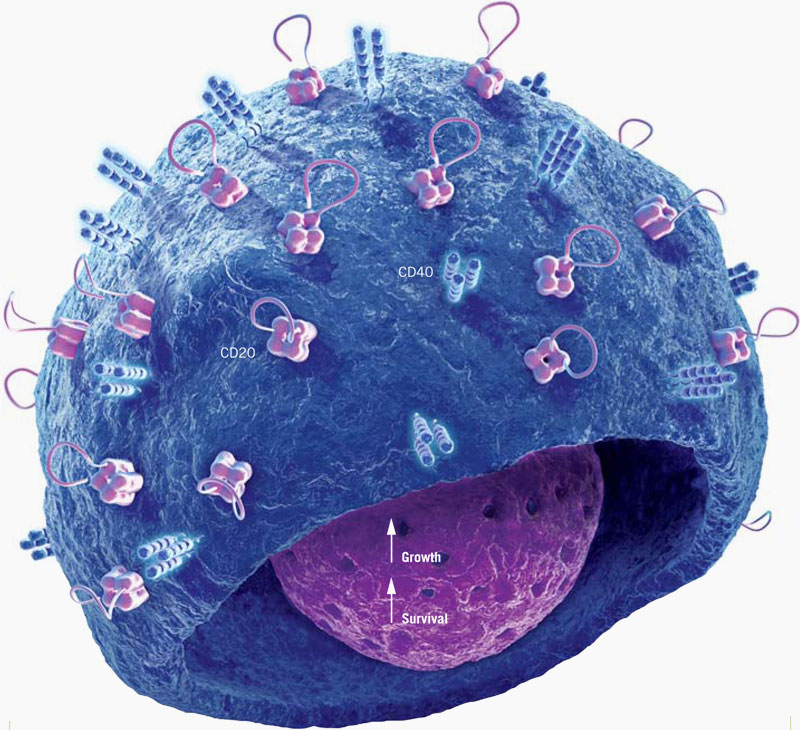
\includegraphics[height=50mm]{Cover/coverimage}  \end{center} % gráficos
~\\ \vspace{5mm}
\begin{centering}
\normalsize Instituto Superior de Estatística e Gestão de Informação\\
\normalsize Universidade Nova de Lisboa
\\ \vspace{30mm}
\large \textbf{PROGRAMAÇÃO GENÉTICA APLICADA A PREVISÃO DE PARÂMETROS FARMACOCINÉTICOS}
\\ \vspace{10mm}
\normalsize por
\\ \vspace{10mm}
\large Dizando Norton António Mvemba (M2012341) % e à previsão do ano de lançamento de músicas
\\ \vspace{30mm}
\setstretch{1.5}
\normalsize Trabalho de projeto apresentado como requisito parcial para a obtenção do grau de Mestre em Gestão de Informação, 
Especialização em Gestão do Conhecimento e Business Intelligence
\\ \vspace{30mm}

\begin{tabular}{c}
\setstretch{1.5}
\normalsize{Orientador: Leonardo Vanneschi, Ph.D} \\
\normalsize{Co-Orientador: Mauro Castelli, Ph.D} \\
\end{tabular}
 
\vspace{25mm}

%\Large \textbf{\todaythesis\today} \\
\normalsize Abril de 2014 \\
\end{centering}
\let\thepage\relax
%\end{flushleft}
\pagebreak


\clearpage
% Since I am using double sided pages, the second page should be white.
% Remember that when delivering the dissertation, IST requires for the cover to appear twice.

\thispagestyle{empty}
\cleardoublepage

\setcounter{page}{1} \pagenumbering{roman}

\baselineskip 18pt % line spacing: -12pt for single spacing
                   %               -18pt for 1 1/2 spacing
                   %               -24pt for double spacingnts}